\documentclass[UTF8]{ctexart}
\usepackage{geometry}
\usepackage{enumerate}
\usepackage{amsmath}
\usepackage{graphicx}
\usepackage{subcaption}
\title{数据挖掘中期报告}
\date{}
\author{第28组-平凡的矿工}


\begin{document}
\maketitle
\section{总述}
本次中期报告主要介绍任务一(有监督学习)遇到的问题,采取的解决办法和模型的尝试。数据处理过程中,我们采用了“分解大文件”的方案解决大批数据的问题;在训练过程中,我们尝试了DNN, LSTM模型。
\section{数据处理}
\subsection{label的生成}
我们本次的任务分为两个部分:时序性预测和非时序性预测。假设当前时间是t, 时序性预测是通过$t-t_0:t$的features预测$t+n$的labels; 非时序性预测是仅通过$t$时刻的features预测$t+n$时刻的labels。我们设置$t_0=20$, $n=10$。
\subsection{面临的问题}
由于这次的数据量比较大(1.64GB),我们考虑到了训练过程中内存溢出的可能性。实际上根据其他小组同学的反馈,将全部数据导入内存确实存在内存占用过多的现象。因此,如何在有限的内存量下完成大数据量的导入和训练成为了数据处理的主要问题。
\subsection{解决办法}
我们考虑将大文件进行分解成若干个小文件的方法进行处理,这样训练的时候只需顺序加载小文件即可。分解小文件的过程虽然需要将大文件全部加载入内存,但是由于不涉及模型的训练,因此内存占用并不大。实际实验证明这个方法是可行的,而且不会损失太多数据。
\section{模型训练}
\subsection{非时序性预测}
我们采用了多层DNN的模型,网络结构如下
\begin{verbatim}
    Layer (type)                 Output Shape              Param #   
    =================================================================
    batch_normalization_v1 (Batc (None, 137)               548       
    _________________________________________________________________
    dense (Dense)                (None, 1000)              138000    
    _________________________________________________________________
    dropout (Dropout)            (None, 1000)              0         
    _________________________________________________________________
    dense_1 (Dense)              (None, 500)               500500    
    _________________________________________________________________
    dropout_1 (Dropout)          (None, 500)               0         
    _________________________________________________________________
    dense_2 (Dense)              (None, 1)                 501       
    =================================================================
    Total params: 639,549
    Trainable params: 639,275
    Non-trainable params: 274
    _________________________________________________________________

\end{verbatim}
\subsection{时序性预测}
我们尝试了LSTM的模型,网络结构如下
\begin{verbatim}
    _________________________________________________________________
    Layer (type)                 Output Shape              Param #   
    =================================================================
    cu_dnnlstm (CuDNNLSTM)       (None, 50)                37800     
    _________________________________________________________________
    dense_3 (Dense)              (None, 1)                 51        
    =================================================================
    Total params: 37,851
    Trainable params: 37,851
    Non-trainable params: 0
    _________________________________________________________________
\end{verbatim}
\subsection{训练结果和遇到的问题}
总体来说采用LSTM进行非时序性预测的结果还是比较满意的,因为利用了时序性的信息。但是采用DNN会出现Loss震荡的问题
\subsubsection{训练速度慢的问题}
一开始我们采用了直接将一个csv大文件分解为几个小的csv文件的问题来解决,这个过程是使用pandas执行的,但是实际训练中的速度还是比较慢,于是我们测试了从数据加载到送入模型过程中各个过程使用numpy和使用pandas所用的时间比例\\
\begin{table}[!htbp]
    \centering
    \begin{tabular}{|c|c|c|}
        \hline
        读取数据 & 提取特征 & 分解minibatch \\
        \hline
        82.7\% & 16.2\% & 1.1\% \\
        \hline
    \end{tabular}
    \caption{使用pandas读取数据}
\end{table}
\begin{table}[!htbp]
    \centering
    \begin{tabular}{|c|c|c|}
        \hline
        读取数据 & 提取特征 & 分解minibatch \\
        \hline
        35.7\% & 60.2\% & 4.1\% \\
        \hline
    \end{tabular}
    \caption{使用numpy读取数据}
\end{table}
通过实验发现采用numpy可以有效提高数据处理的速度。
\subsubsection{Loss震荡的问题}
DNN的训练效果不是很理想,由于是regression任务我们只能通过validation\_loss来判断训练情况, 如图是使用DNN训练的过程中的典型情况。
\begin{figure}[h]
    \centering
    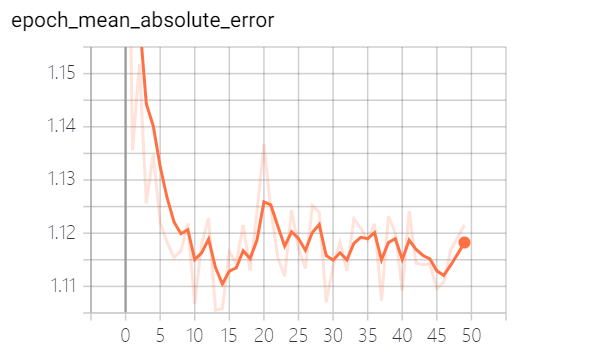
\includegraphics[]{result.png}
    \caption{DNN测试集Loss}
\end{figure}
不管参数如何调整,训练到一定程度loss会剧烈震荡。我们采取了添加标准化层和添加正则化项等尝试,但是效果并不是太明显,我们目前推测是与训练特征的分布有关,但是由于时间原因还没有进一步的实验。
\section{下阶段任务}
下一阶段任务主要有:\\
\begin{enumerate}
    \item 改善网络结构,改善任务一的预测精确度。同时尝试CNN,GBDT等算法,比较试验结果
    \item 完成任务二和任务三。
\end{enumerate}

\end{document}
